\chapter{T-Cells, Calcium Concentration}
\label{chapter:t-cell}

Lymphocytes form a key component of the immune system. T cells are a type of lymphocyte and are responsible for responding to viruses, fungi, allergens and tumors. Different subtypes of t cells exist, that fulfill various responsibilities. They are transported throughout the body via the lymphatic system and blood.\cite{Kumar2018}

Precursor cells are formed in the bone marrow. Once they are transported to the thymus they undergo maturation and selection to become t cells. Each cell forms receptors, called t cell receptors (TCR), that respond to one perticular out of many ($10^6 - 10^9$) possible short pieces of proteins, called peptides. These peptides are attached to the major histocompatibility complex (MHC) present on antigens and antigen presenting cells (APC). Important aspects of the selection are ensuring that the t cells react to foreign peptides, but not to those present on the body's own cells.\cite{Ashby2024}

In positive selection cells in the thymus present peptides on their MHC. If a t cell is unable to bind, it will undergo apoptosis, a type of cell death. T cells which were able to bind recieve survival signals. Negative selection verifies that t cells will not attack the body's own cells. This is done by only selecting t cells which only bind moderatly to the peptides presented, as a strong bond sugessts that these t cells would have a high likelihood of being reactive to own cells.\cite{Hagel2018} If a t cell passed both the positive and negative selection it is transported to the periphery.

There are multiple types of peripheral t cells. Native t cells respond to new antigens. Cytotoxic t cells kill cells which present peptides on their MHC compatible with the t cells TCR. Helper T cells activate other parts of the immune response. Memory t cells shorten the reaction time when the same antigen is encountered again at a later point in time. Suppressor t cells moderate the immune response.\cite{Ganong1997}

\section{Components of a T-Cell}

\begin{comment}
	t cell:
	- t cell receptor
	- co-stimulator
	- ER
	- \Calcium permiable ion channel on the ER
	- \Calcium storage in the ER
	- cytoplasm
	- STIM
	- plasm membrane
	- \Calcium release activated \Calcium channel (CRAC)
	- (cytoskeleton)
	- (nucleus)
	
	apc:
	- MHC
	- co-stimulator
\end{comment}


\begin{figure}
	\centering
	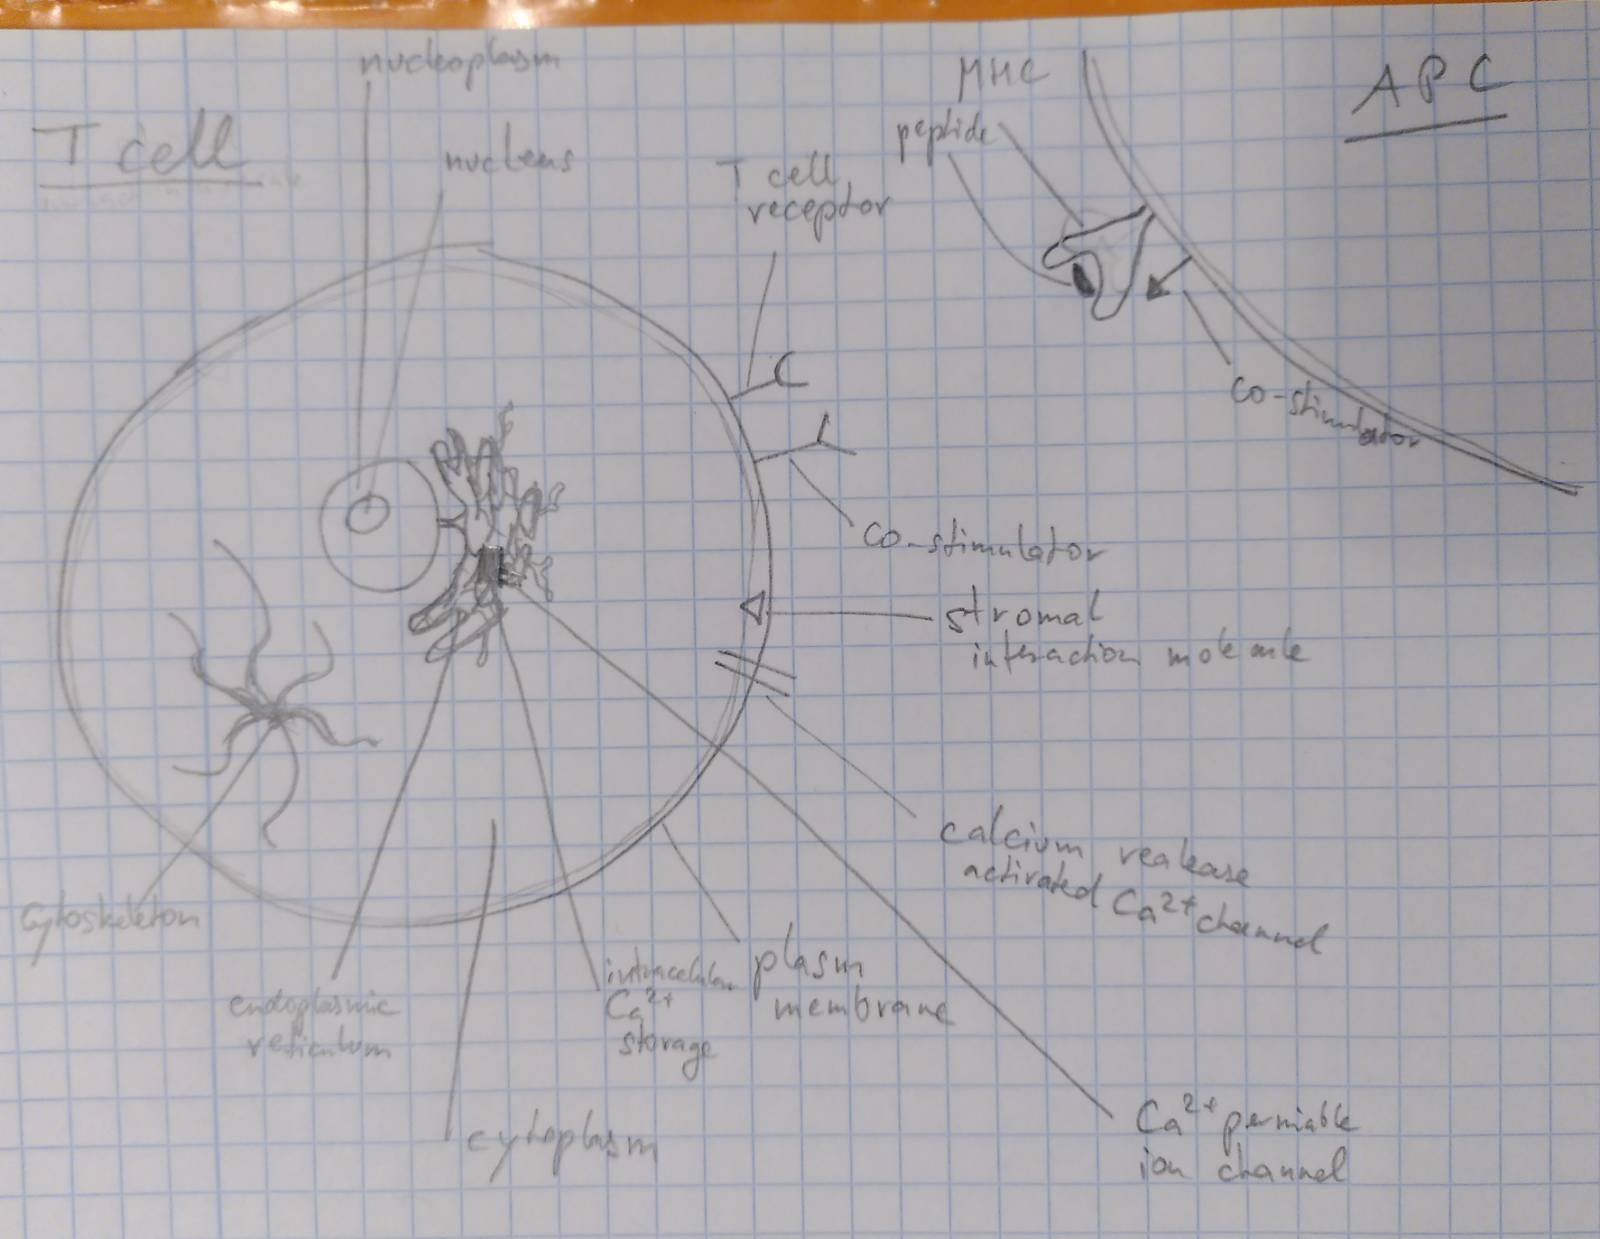
\includegraphics[width=0.7\linewidth]{fig/tmp_t_cell_components}
	\caption{Skematic view of a t cell and antigen presenting cell, with all relevant components.}
	\label{fig:tcellcomponents}
\end{figure}

\section{Activation}

Activation is necessary for t cells to divide and perform their functions.\cite{Ganong1997}

When a native t cell encounters an APC that is compatible, a bond is formed between the TCR on the t cell and the peptide-MHC complex on the APC. This recognition can be triggered by less than ten molecules of foreign substance and is therefore described as near perfect. Sufficiently long contact is nececcary between the APC and the t cell in order for the t cell to activate. The role of contact time in t cell activation is modelled by Morgan et.al.\cite{morgan2023}.

The presence of co-stimulatory molecules is needed for proper activation. The bond between the co-stimulatory molecules on the t cell and APC plays a role in signaling. \Calcium signals play a vital part in t cell activation.

An increase of \Calcium in t cells during activation is caused by the stimulation of \Calcium permiable ion channel receptors on the ER membrane. \Calcium is released from the ER into the cytoplasm. Additionally this decrease in \Calcium is sensed by STIM, which leads to an influx of \Calcium through plasma membrane CRAC channels.\cite{smith2009}

As the intracellular \Calcium concentration is dependent on the interaction between \Calcium sources and sinks, a variety of different forms in \Calcium concentration have been observed. Examples are infrequent spikes, sustained oscilations and plateaus.\cite{Lewis2001}

Intercellular \Calcium increase together with other signals lead to a redistribution of receptors, signaling molecules and organelles.\cite{joseph2014}
